%\documentclass[10pt]{letter}
%\usepackage[utf8]{inputenc}

%%%%%%%%%%%%%%%%%%%%%%%%%%%%%%%%%%%%%%%%%%%%%%%%%
% compile with LuaLatex
%%%%%%%%%%%%%%%%%%%%%%%%%%%%%%%%%%%%%%%%%%%%%%%%%%%%%%%
\documentclass[11pt]{report}
\usepackage{epsfig}
\usepackage{amssymb,amsmath,amsfonts}
\usepackage[activeacute,american]{babel}
%\usepackage[utf8]{inputenc}
\usepackage{subfiles}
\usepackage{cite}
\usepackage{csquotes}
\usepackage{esvect}
\usepackage[acronym,nonumberlist]{glossaries}
\renewcommand{\acronymname}{Nomenclature}
\usepackage{multicol}
\usepackage{caption} 
\usepackage{float}
\usepackage[
    math-style=ISO,      % Upper Case Greek is in italics
    bold-style=ISO,      % Bold math is in italics
    partial=upright,     % nabla and partial upright
    nabla=upright,
  ]{unicode-math}
\topmargin 1.2cm 
\textwidth 16.1cm
\textheight 22.5cm
\oddsidemargin 0.7cm
\setcounter{tocdepth}{5}
\addtolength{\voffset}{-2.4cm}
\addtolength{\hoffset}{-0.5cm}
\usepackage{booktabs}
\usepackage{setspace}
\usepackage{mathtools}
%\doublespacing
\onehalfspacing
\usepackage{caption}
 \captionsetup[figure]{labelfont={bf},name={Figura},labelsep=period}


%%%%%%%%%%%%%%%%%%%%%%%%%%%%%%% 
% citas
% \footnotetext{Mott, Robert L. Mecanica de Fluidos 6/e. Pearson educación, 2006.}
% \footnotetext{Pritchard, Philip J. Fox and McDonald’s Introduction to Fluid Mechanics (8th ed.). John Wiley $\&$ Sons. (2011).}
% \footnotetext{Munson, Bruce R., et al. "Fundamentals of Fluid Mechanics, John Wiley $\&$ Sons." Inc., USA (2006).}
%%%%%%%%%%%%%%%%%%%%%%%%%%%%%%% 

%%%%%%%%%%%%%%%%%%%%%%%%%%%%%%%%%
\begin{document}
\centering{ \textbf{\Large{Mec\'anica de fluidos}}}

\centering {\Large{2$^\circ$ semestre 2020: 541209-1}}
\vspace{1cm}

\flushleft{ \large \underline{\textbf{Pr\'actica 8: Flujos compresibles}}}

%%%%%%%%%%%%%%%%%%%%%%%%%
\vspace{1cm}

\underline {Problema 1:}
\vspace{0.2cm}

Se tiene para una onda de choque estacionaria:
\begin{itemize}
\item $p_1=80$\,kPa
\item $T_1=5$\,$^\circ$C $= 278.5$\,K
\item $V_1=600$\,m/s
\end{itemize}
Determine las condiciones de flujo aguas abajo.
\vspace{0.2cm}

\underline{\textbf{Respuesta:}}

Para calcular las condiciones de flujo aguas abajo, utilizaremos las ecuaciones para ondas de choque normales (Ap\'endice de flujos compresibles). Estas ecuaciones relacionan el n\'umero de Mach $Ma_1$ del flujo en el punto previo a la onda de choque (punto 1) el cual \textbf{debe} ser supers\'onico (en caso contrario, no se podr\'a formar una onda de choque), $Ma_2$ el n\'umero de Mach $Ma_2$ del flujo en el punto posterior a la onda de choque el cual \textbf{debe} ser subs\'onico, y las propiedades del fluido en ambos puntos. Primero, en base a las propiedades del flujo ya conocidas, calcularemos $Ma_1$:


$$
M a_{1}=\frac{V_{1}}{C_{1}}=\frac{V_{1}}{\sqrt{K R T}}=\frac{600 \mathrm{~m/s}}{\sqrt{1.4 \cdot 286.9 \frac{N m}{\mathrm{kg\cdot K}} \cdot 278.5 \mathrm{K}}}=\frac{600 \mathrm{~m}/ \mathrm{s}}{334.6 \mathrm{~m} / \mathrm{s}}=1.79
$$
Ya que $Ma_1>1$, el flujo es supers\'onico y cumplimos con que el flujo debe ser supers\'onico en el punto previo a la onda de choque. \textit{nota: para aire $k=1.4$ y $R=286.9\frac{N m}{\mathrm{kg\cdot K}}$}.

Ya conocido $Ma_1$, podemos calcular las propiedades del flujo en el punto posterior a la onda de choque normal:


$$
M a_{2}^{2}=\frac{(k-1) M a_{1}^{2}+2}{2 k Ma_{1}^{2}-(k-1)} \quad \stackrel{\text { aire }}{\longrightarrow} \quad M_{a_{2}}=\sqrt{\frac{0.4 Ma_{n}^{2}+2}{2.8 M a_{1}^{2}-0.4}}=0.62
$$
El flujo en el punto $2$ es subs\'onico (por supuesto, ya que $Ma_1>1$ siempre obtendremos $Ma_2<1$ al utilizar esta relaci\'on)

$$
\begin{array}{r}
\displaystyle \frac{p_{2}}{p_{1}}=\frac{1}{k+1}\left(2 k M_{a_{1}}^{2}-(k-1)\right) \stackrel{\text { aire }}{\longrightarrow} \frac{p_{2}}{p_{1}}=\frac{1}{2.4}\left(2.8 \mathrm{Ma}_{1}^{2}-0.4\right)=3.57 \\
\Rightarrow p_{2}=3.57 \cdot p_{1}=3.57+80 \mathrm{kPa}=285.6 \mathrm{kPa}
\end{array}
$$

$$
\begin{array}{r}
\displaystyle \frac{T_{2}}{T_{1}}=\left[2+(k-1) M a_{1}^{2}\right] \frac{2 Ma^{2}-(k-1)}{(k+1)^{2} M_{a_{1}}^{2}} \stackrel{aire}{\rightarrow}\left[2+0.4 Ma_{1}^{2}\right]\left[\frac{2.6 Ma_{1}^{2}-0.4}{(2.4)^{2} Ma_{1}^{2}}\right] \\ 
\displaystyle  \Rightarrow \frac{T_{2}}{T_{1}}=1.524 \\ 
\displaystyle \Rightarrow T_{2}=T_{1} \cdot 1.524=1.524 \cdot 278.5 \mathrm{k}=424.4 \mathrm{k}
\end{array}
$$

La densidad del aire en ambos puntos puede ser calculada utilizando la ecuacion que relaciona el cambio de densidad a trav\'es de una onda de choque en conjunto con la ecuaci\'on de gases perfectos o utilizando la ecuaci\'on de gases perfectos para ambos puntos por separado:
$$
\rho_{1}=\frac{p_{1}}{R T_{1}} \quad \text{y} \quad p_{2}=\frac{p_{2}}{R T_{2}}
$$
\textbf{Un par de alternativas a evaluar las distintas expresiones presentadas corresponden a obtener los valores correspondientes a partir de los valores tabulados en el ap\'endice de flujos compresibles e interpolar en caso de que no se encuentre el valor deseado o tambien a partir del gr\'afico correspondiente (tambien presentado en el ap\'endice)} 
%Estas ecuaciones relacionan el n\'umero de Mach en alg\'un punto con las propiedades del fluido y las propiedades de estancamiento en ese punto. Primero, calcular




%%%%%%%%%%%%%%%%%%%%%%%%%
\newpage
%%%%%%%%%%%%%%%%%%%%%%%%%

\underline {Problema 2:}
\vspace{0.2cm}

Determine el fluijo m\'asico m\'aximo admisible para la tobera de la figura ~\ref{fig:fig1} y la presi\'on en el plano de salida cuando se tiene flujo estrangulado
\begin{figure}[H]
\centering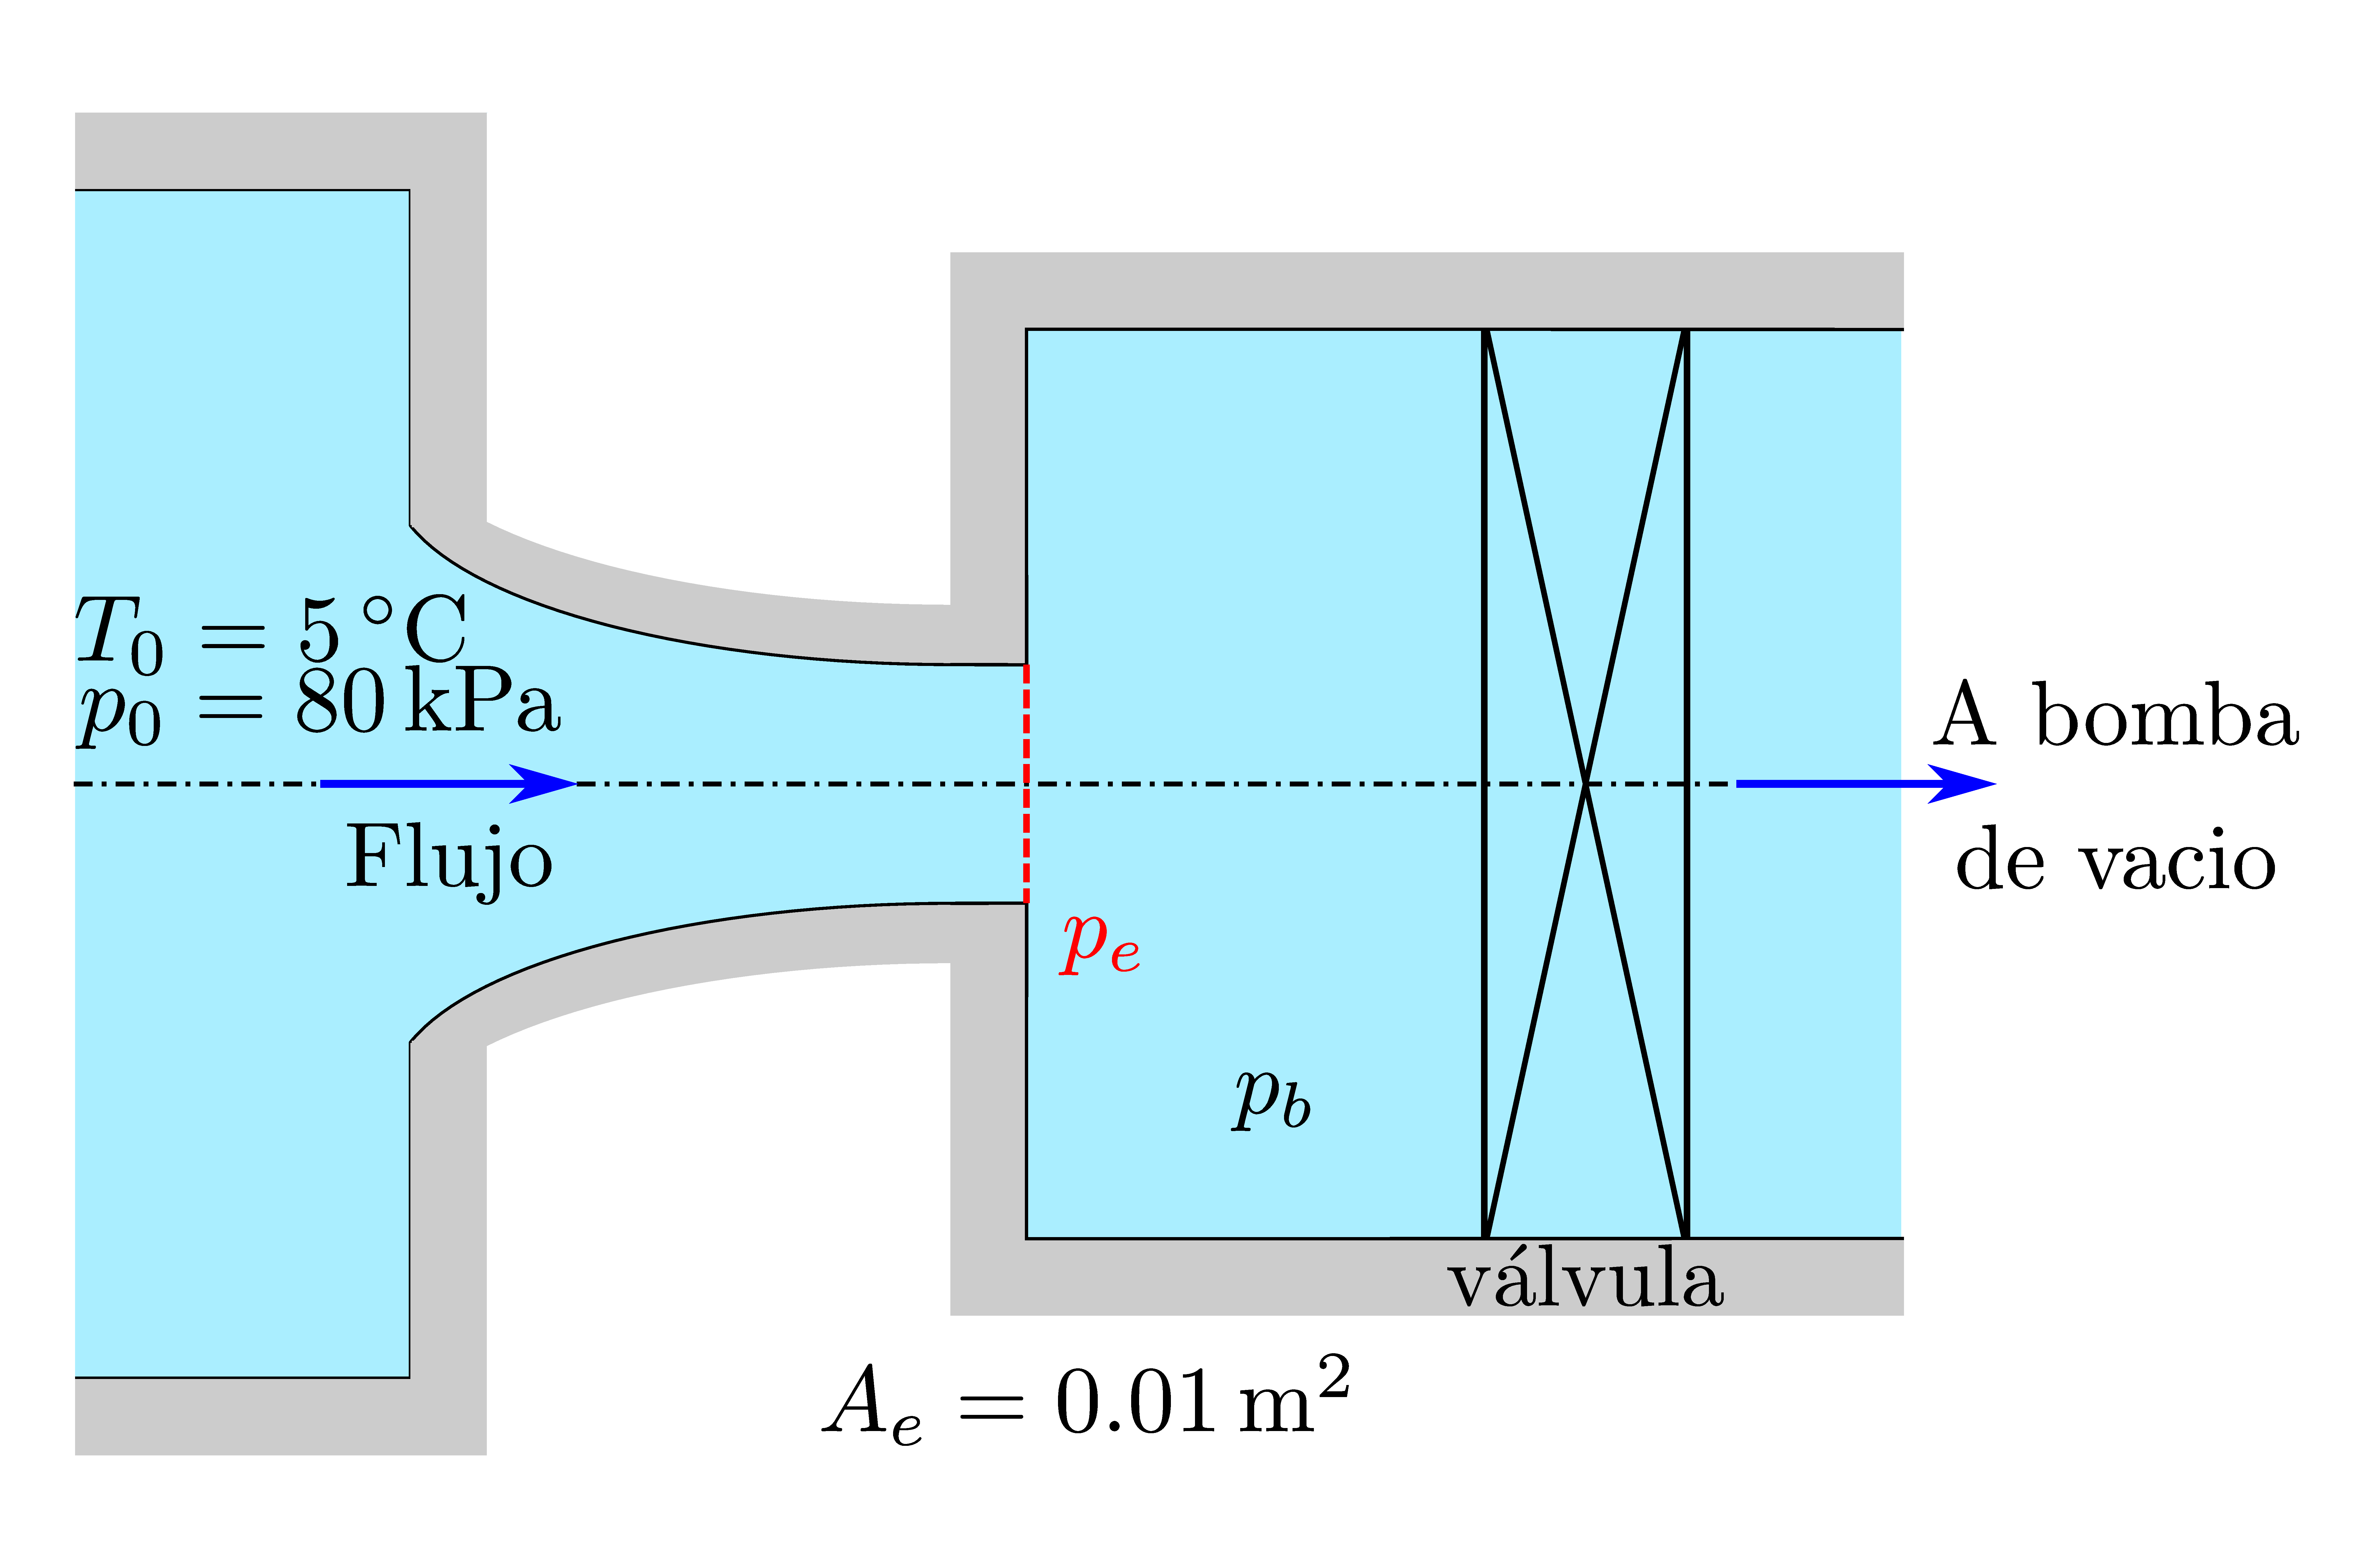
\includegraphics[width=0.8\textwidth]{Figures/tobera_conv.eps}
\caption{\label{fig:fig1} }
\end{figure}
\vspace{0.2cm}

\underline{\textbf{Respuesta:}}

El flujo m\'asico m\'aximo se puede obtener a partir de la condici\'on cr\'tica para toberas, la cual indica que el m\'aximo valor para $Ma$ en la secci\'on de menor \'area del conducto (garganta) debe ser igual a $1$. Para toberas convergentes, la garganta coincidir\'a con el plano de salida, mientras que para toberas convergente-divergentes no. El flujo m\'asico m\'aximo puede ser obtenido  a partir de la siguiente relaci\'on:

$$
\dot{m}_{\max }=0.6847 A^{*} \rho_{0}\left(R T_{0}\right)^{1 / 2}=\frac{0.6847 p_{0} A^{*}}{\left(R T_{0}\right)^{1 / 2}}
$$
Como el \'area cr\'itica (aquella requerida para que $Ma=1$) estar\'a determinada por el conducto ($A^{*}=A_e$), podemos evaluar la expresi\'on anterior. con:

$$
\begin{array}{l}
p_{0}=80 \mathrm{kPa} \\
T_{0}=5^{\circ} \mathrm{C}=278.3 \mathrm{~K}\\
A_e=0.01 \text{m}^2
\end{array}
$$
Obtendremos:
$$
\dot{m}_{\max }=\frac{0.684\cdot80 \mathrm{kPa} \cdot 0.01 \mathrm{~m}^{2}}{\left(286.9 \frac{\mathrm{J}}{\mathrm{kg}\cdot\mathrm{K}} \cdot 278.3 \mathrm{K}\right)^{\mathrm{1/2}}}
$$

$$
\dot{m}_{max}=1.94 \mathrm{~kg} / \mathrm{s}
$$
La presi\'on en el plano de salida puede ser obtenida considerando que el flujo est\'a estrangulado (la presi\'on en el plano de salida deber\'a ser igual a la presi\'on cr\'itica). \textit{Nota: para toberas convergente-divergentes la presi\'onm cr\'itica para flujo estrangulado se alcanzar\'a en la garganta, que no coincide con el plano de salida}. Entonces:
$$
\left(\frac{p_{e}}{p_{s}}\right)_{\text {estrangulado}}=\frac{p^{*}}{p_{0}}=\left(\frac{2}{k+1}\right)^{k /(k-1)}=\left(\frac{2}{2.4}\right)^{1.4 / 0.4}=0.528
$$
\textit{Nota: la raz\'on $p^*/p_0$ siempre tendr\'a un valor igual a $0.528$ para aire.} 

%\textbf{Nota2: Todas las propiedades calculadas a partir de las expresiones mencionadas en este problema (con excepci\'on de $Ma$) pueden ser obtenidas a partir de las tablas del ap\'endice de flujos compresibles}
%%%%%%%%%%%%%%%%%%%%%%%%%
\newpage
%%%%%%%%%%%%%%%%%%%%%%%%%
\underline {Problema 3:}
\vspace{0.2cm}

Determine las condiciones de flujo en $2$ y $3$ para la tobera representada en la figura~\ref{fig:fig2}. Considere que el flujo es isoentr\'opico en toda la tobera y no se forman ondas de choque.

\begin{figure}[H]
\centering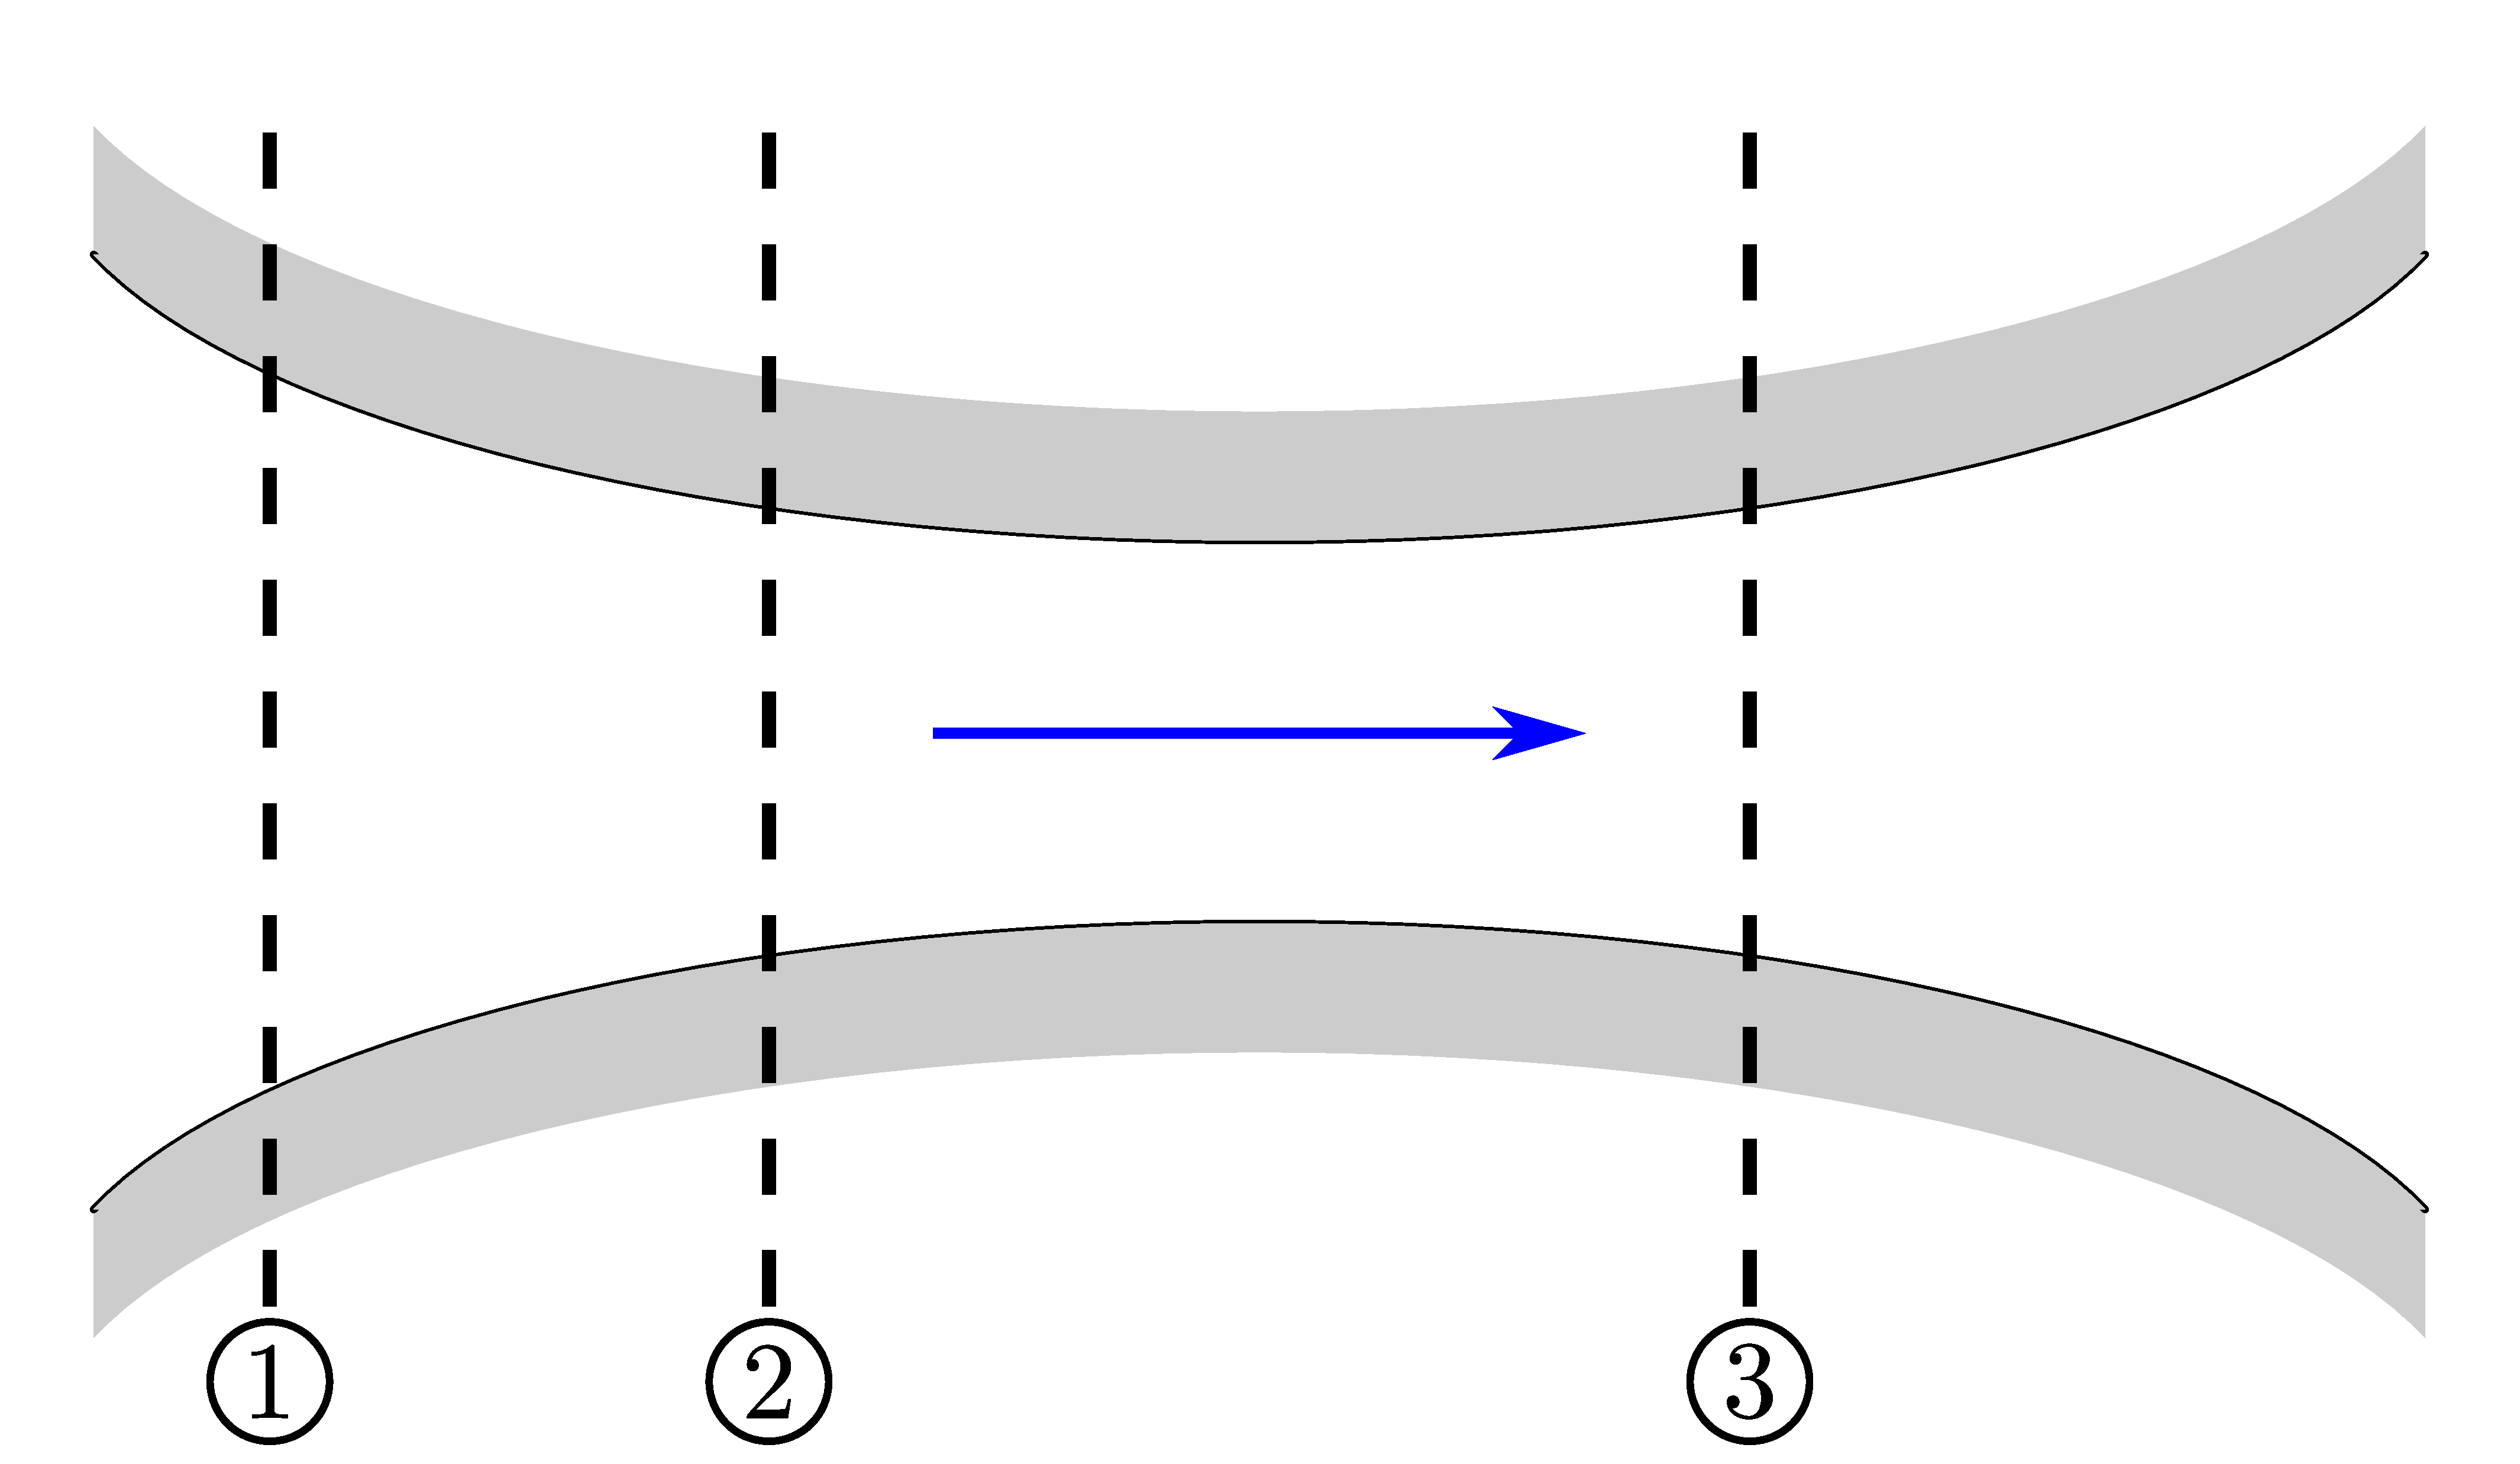
\includegraphics[width=0.5\textwidth]{Figures/conv_div.eps}
\caption{\label{fig:fig2} }
\end{figure}
Considere:
\begin{itemize}
\item $V_1=180$\,m/s
\item $p_1=500$\,kPa
\item $T_1=470$\,K
\item $A_1=0.05$\,m$^2$
\item $A_2=A_3=0.036$\,m$^2$
\item El flujo en $3$ es supers\'onico
\end{itemize}
\vspace{0.2cm}

\underline{\textbf{Respuesta:}}
a) Condiciones de flujo en $2$

Primero debemos determinar las propiedades de estancamiento. Para esto, calcularemos $Ma_1$ y calcularemos las propiedades de estancamiento en $1$ a partir de las propiedades en este punto (las cuales ya son conocidas):

$$
M a_{1}=\frac{V_{1}}{c_{1}}=\frac{V_{1}}{\sqrt{k R T_{1}}}=0.415
$$
ya que $Ma_1<1$, el flujo previo a la garganta \textbf{debe} ser supers\'onico (incluyendo al punto $2$). Las propiedades de estancamiento pueden ser obtenidas a partir de las relaciones para gases ideales:

$$
\frac{T_{0_1}}{T_{1}}=\left(1+\frac{k-1}{2} Ma_1^{2}\right) \Rightarrow T_{0_1}=486.2 \mathrm{k}
$$

$$
\frac{p_{0_1}}{p_{1}}=\left(1+\frac{k-1}{2} Ma_1^{2}\right)^{k(k-1)} \Rightarrow p_{0_1}=563 \mathrm{kPa}
$$
El \'area cr\'itica se calcula mediante:
$$
\frac{A_{1}}{A_1^{*}}=\frac{\left(1+0.2 Ma_{1}^{2}\right)^{3}}{1.728 Ma_1}=1.544
$$
$$
\Rightarrow A^{*}=0.0323 \mathrm{~m}^{2}
$$
Ya conocidas las propiedades de estancamiento en $1$, supondremos que (ya que no existe onda de choque) el flujo es isoentr\'opico en toda la tobera. Entonces, las propiedades de estancamiento y el \'area cr\'itica en $2$ ser\'an iguales que las propiedades de estancamiento en $1$:
$$
\begin{array}{l}
T_{0_1}=T_{0_2} \\
p_{0_1}=p_{0_2} \\
A^*_1=A^*_2
\end{array}
$$
Al "extrapolar" estas propiedades, podremos calcular las propiedades de flujo en $2$ a partir de las relaciones para propiedades de estancamiento para gases ideales. Primero determinaremos $Ma_2$ a partir de la relaci\'on de \'area cr\'itica (conocemos $T_{0_2}$, $p_{0_2}$, $A^*_2$ y $A_2$, necesitamos: $Ma_2$, $T_{2}$, $p_2$):
$$
\frac{A_{2}}{A^{*}}=\frac{\left(1+0.2 M a_{2}^{2}\right)^{3}}{1.728 M a_{2}}
$$
$$
\frac{A_{2}}{A^{*}}=\frac{0.036 m^{2}}{0.0323 m^{2}}=1.115=\frac{\left(1+0.2 M a_{2}^{2}\right)^{3}}{1.728 Ma_{2}}
$$
Al resolver esta ecuaci\'on no lineal, debemos asegurarnos que la raiz obtenida sea menor a $1$ (el flujo en este punto \textbf{debe} ser subs\'onico). Considerando este requerimiento obtendremos:

$$
Ma_{2}=0.673
$$
Conocido $Ma_2$ podemos calcular el resto de las propiedades utilizando las relaciones para propiedades de estancamiento:
$$\frac{T_{0}}{T_{2}}=1.091 \rightarrow T_{2}=445.6 K$$

$$
\frac{P_{0}}{P_{2}}=1.355 \rightarrow P_{2}=415.5 \mathrm{kpa}
$$
adem\'as, podemos calcular la velocidad de flujo:
$$
V_{2}= Ma_{2} \cdot c=Ma_{2} \sqrt{k R T_{2}} 
$$
$$
 \Rightarrow v_{2}=284.5 \mathrm{~m} / \mathrm{s}
$$

b) Condici\'on de flujo en $3$

Para obtener las propiedades del flujo en este punto, realizaremos el mismo procedimiento que para el punto $2$, pero ahora consideraremos que el flujo debe ser supers\'onico. Entonces:

$$
\frac{A_{3}}{A^{*}}=\frac{\left(1+0.2 Ma_{3}^{2}\right)^{3}}{1.728 Ma_{3}}
$$
$$
\frac{0.036}{0.0323}=\frac{\left(1+0.2 {Ma}_{3}^{2}\right)^{3}}{1.728 {Ma}_{3}}
$$
Al resolver esta ecuaci\'on no lineal, ahora deberemos asegurarnos que la raiz obtenida sea mayor a $1$ (para que el flujo sea supers\'onico). Al considerar este requerimiento obtendremos:

$$
{Ma}_{3}=1.4
$$
y el resto de las propiedades a partir de este valor:
$$
\frac{P_{0}}{P_{3}}=3.1823 \Rightarrow P_{3}=1.769 \text { lepa }
$$
$$
\frac{T_{2}}{13}=1.392 \rightarrow T_{3}=349.3 \mathrm{k}
$$
\textbf{Nota: Todas las propiedades calculadas a partir de las expresiones mencionadas en este problema (con excepci\'on de $Ma$) pueden ser obtenidas a partir de las tablas del ap\'endice de flujos compresibles}
%%%%%%%%%%%%%%%%%%%%%%%%

\newpage
\underline {Problema 4:}
\vspace{0.2cm}

Para la tobera presentada en la figura~\ref{fig:fig3} determine:
\begin{enumerate}
\item Condici\'on de diseño
\item Presi\'on m\'axima requerida para que exista flujo supers\'onico en la zona divergente
\item Presi\'on m\'inima requerida para que se formen ondas de choque normales
\item Condiciones de flujo en el plano de salida si $p_b=50$\,kPa. Adem\'as, condiciones de flujo antes y despues de la onda de choque y el \'area transversal de la onda de choque.
\end{enumerate}

\begin{figure}[H]
\centering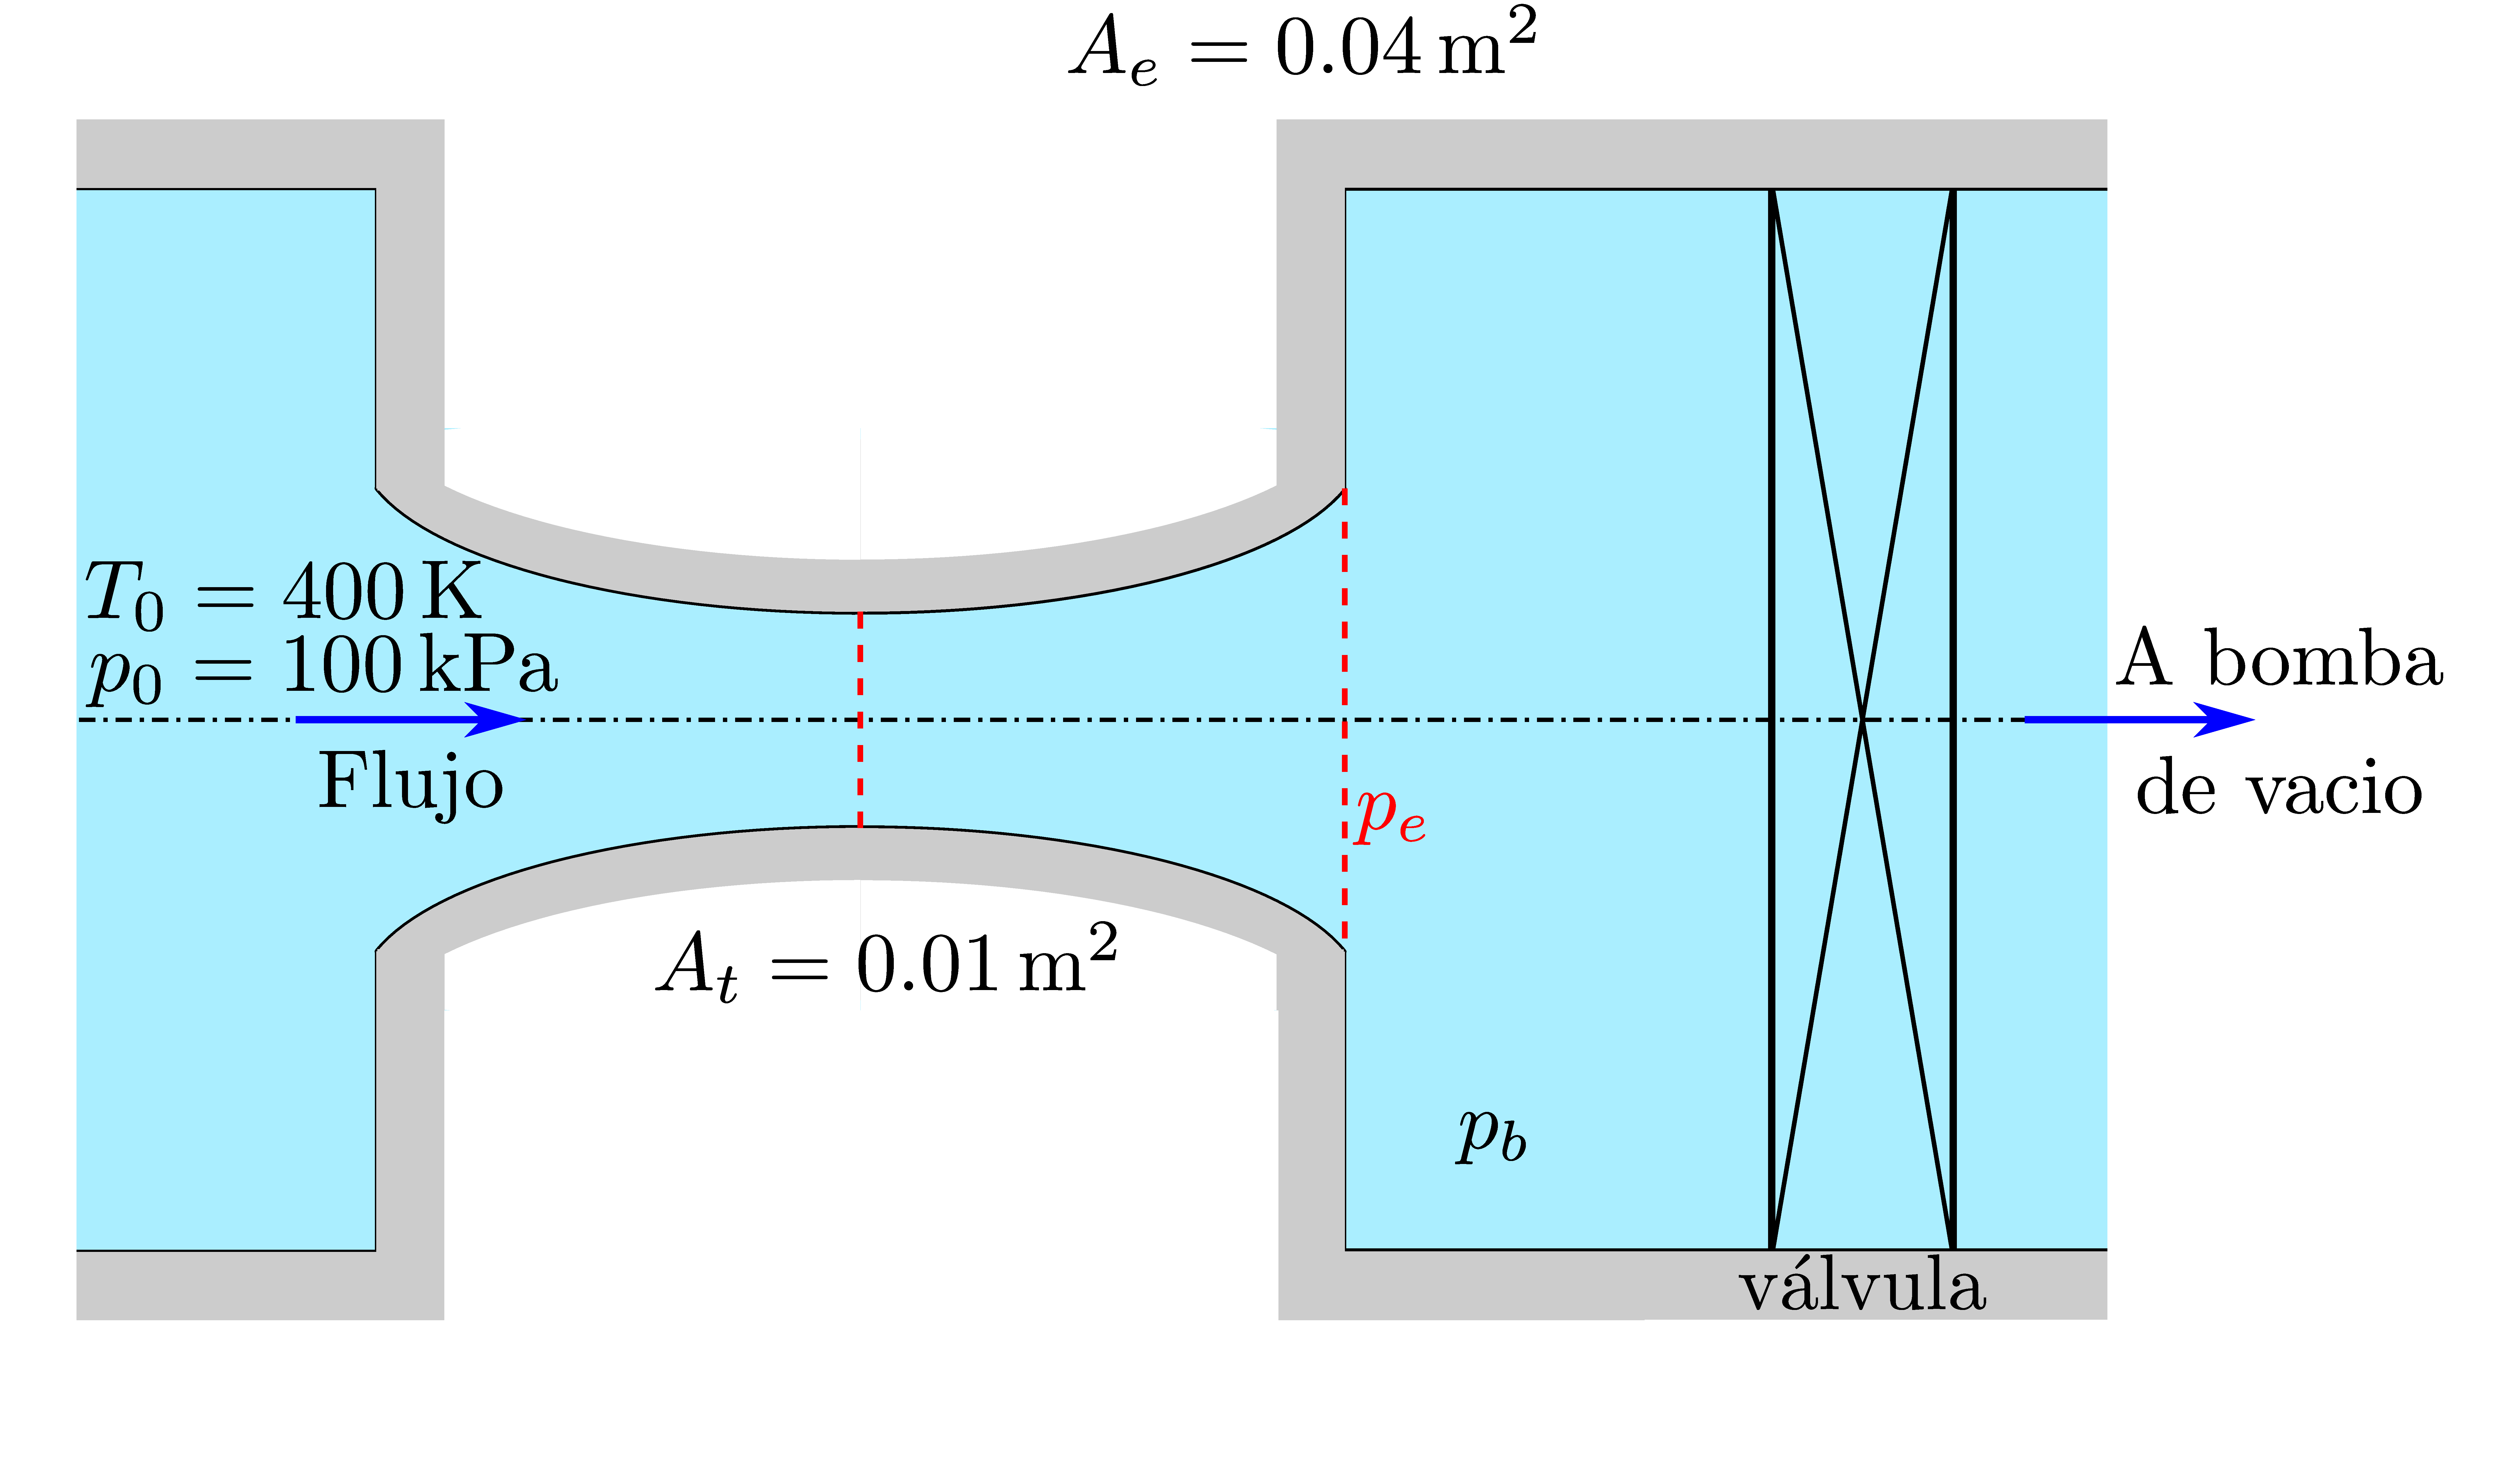
\includegraphics[width=0.8\textwidth]{Figures/tobera_convdiv.eps}
\caption{\label{fig:fig3} }
\end{figure}

\vspace{0.2cm}

\underline{\textbf{Respuesta:}}


a) Condici\'on de diseño.

La condici\'on de diseño ser\'a aquella para la que podremos obtener flujo supers\'onico posteriormente a nuestra tobera. Para que esto se cumpla no deber\'a haber ondas de choque en ningun punto. Es decir, el flujo ser\'a isoentr\'opico en toda la tobera y la presi\'on en el plano de salida $p_e$ deber\'a ser igual a la presi\'on en el reservorio de la derecha $p_b$ (esta \'ultima igualdad asegura que no se formar\'an ondas de choque oblicuas o de expansi\'on en la zona posterior a la tobera). Ya que el flujo es isoentr\'opico en toda la tobera:
$$
\begin{array}{l}
p_{0}=p_{0_e} \\
T_{0}=T_{0_{e}} \\
A^{*}=A_{e}^{*}=A_{t}=0.01 \mathrm{~m}^{2}
\end{array}
$$
Para obtener $Ma_e$, utilizaremos la relaci\'on para \'area cr\'itica:
$$
\frac{A_{e}}{A^{*}}=\frac{0.04 \mathrm{~m}^{2}}{0.01 \mathrm{~m}^{2}}=4=\frac{\left(1+0.2 \mathrm{Ma_e}^{2}\right)^{3}}{1.728 \mathrm{Ma}_{\mathrm{e}}}
$$
Al resolver esta expresi\'on, deberemos asegurarnos que la raiz obtenida sea mayor a $1$ (la condici\'on de diseño establece que el flujo debe ser supers\'onico). Al considerar este requerimiento obtendremos:
$$
Ma_{e}=2.94
$$
a partir de este valor, podemos obtener la presi\'on en el plano de salida:
$$
\frac{p_{0_e}}{p_{e}}=33.56 \rightarrow p_{e}=2.97 \text{kPa}
$$
y $p_b=p_e=2.97$ kPa debido a la condici\'on de diseño.

\textit{Nota: Si aumentamos la presi\'on $p_b$ se generar\'an ondas de choque oblicuas en la salida de la tobera y si disminuimos $p_b$ se formar\'an ondas de expansi\'on}

\vspace{0.2cm}

b)  Presión máxima requerida para que exista flujo supersónico en la zona divergente. 

Para determinar la presi\'on m\'axima requerida para que exista flujo supers\'onico en alg\'una punto de la zona divergente de la tobera, deberemos considerar primero el comportamiento que tendr\'a el flujo de aire a medida que variamos $p_b$. Si iniciamos con $p_b=p_0$ no habr\'a flujo. A medida que disminuimos $p_b$ ($p_b<p_0$) se generar\'a flujo hacia la derecha. Inicialmente, obtendremos flujo incompresible en toda la tobera. Si disminuimos $p_b$ lo suficiente, la velocidad de flujo aumentar\'a y observaremos efectos de compresibilidad en el flujo, mas este se mantendr\'a a\'un subs\'onico en toda la tobera. Si disminuimos $p_b$  a\'un m\'as podremos llegar al punto en que logremos obtener $Ma_1$ en la garganta. En este punto cr\'itico, inicialmente obtendremos flujo subs\'onico en la zona divergente de la tobera. Adem\'as, hasta este punto, podremos considerar que el flujo en toda la tobera es isoentr\'opico. Si continuamos disminuyendo $p_b$, obtendremos inicialmente flujo supers\'onico en la zona divergente con ondas de choque en la tobera (y posteriormente, flujo con ondas de choque oblicuas posteriores a la tobera, condici\'on de diseño y flujo con ondas expansivas posteriores a la tobera, en ese orden). En resumidas cuentas, para determinar la presi\'on m\'axima $p_b$ requerida para que exista flujo supers\'onico en alg\'un punto, deberemos determinar la presi\'on para la que: 
\begin{itemize}
\item El flujo est\'a estrangulado ($Ma_t=1$)
\item El flujo en la zona divergente es subs\'onico (esto implica adem\'as que el flujo ser\'a subs\'onico en toda la tobera y que no se forman ondas de choque en ning\'un punto)
\item Todo el flujo es isoentr\'opico
\end{itemize}

Considerando el \'ultimo requerimiento, podemos obtener las propiedades de estancamiento y cr\'iticas para el plano de salida:
$$
\begin{array}{l}
p_{0}=p_{0_e} \\
T_{0}=T_{0_{e}} \\
A^{*}=A_{e}^{*}=A_{t}=0.01 \mathrm{~m}^{2}
\end{array}
$$
y a partir de ellas calcular $Ma_2$:
$$
\frac{A_{e}}{A^{*}}=\frac{0.04 \mathrm{~m}^{2}}{0.01 \mathrm{~m}^{2}}=4=\frac{\left(1+0.2 \mathrm{Ma_e}^{2}\right)^{3}}{1.728 \mathrm{Ma}_{\mathrm{e}}}
$$
Al resolver esta expresi\'on, deberemos asegurarnos que la raiz obtenida sea menor a $1$ (ya que establecimos que el flujo debe ser subs\'onico en la zona divergente). Al considerar este requerimiento obtendremos:
$$
M_{a_{e}}=0.1465
$$
El cual podemos utilizar para determinar la presi\'on en el plano de salida a partir de la correspondiente expresi\'on para presi\'on de estancamiento. Entonces:
$$
\frac{p_{0_e}}{p_{e}}=1.015\rightarrow p_{e}=\frac{100 \mathrm{kpa}}{1.015}=98.5 \mathrm{kPa}
$$
Ya que no existen ondas de choque en ning\'un punto (incluyendo el plano de salida):
$$
p_{e}=p_{b}=98.5 \mathrm{kPa}
$$

\vspace{0.2cm}
c) Presi\'on m\'inima requerida para que se formen ondas de choque normales

Para determinar esta presi\'on deberemos considerar que si disminuimos la presi\'on $p_b$ a partir del punto anterior, observaremos que la onda de choque normal se desplazar\'a progresivamente hacia la derecha, hasta que alcanze el plano de salida. A partir de este punto, si disminuimos a\'un m\'as $p_b$, observaremos ondas de choque oblicuas posteriores al plano de salida (luego condici\'on de diseño y despues ondas expansivas posteriores al plano de salida). Entonces, deberemos determinar la presi\'on $p_b$ para la que exista una onda de choque normal en el plano de salida. Es decir, el flujo ser\'a isoentr\'opico hasta este punto (toda la tobera) y luego tendremos una onda de choque normal. Si consideramos la primera condic\'on, podremos determinar $p_e$ de igual forma a que lo hicimos en el punto a (flujo isoentr\'opico en toda la tobera, con flujo supers\'onico en la zona divergente). Entonces:
$$p_e=2.97 \mathrm{kPa}$$
$$Ma_e=2.94$$
La presi\'on $p_b$ estar\'a determinada por el cambio de presi\'on a trav\'es de la onda de choque. Utilizando la expresi\'on correspondiente a este cambio:
$$
\frac{p_{2}}{p_{1}}=\frac{1}{k+1}\left[2 k M a_{1}^{2}-(k-1)\right]
$$
Para esta expresi\'on deberemos considerar que $2$ representa el punto posterior a la onda de choque y $1$ el punto anterior. Entonces:
$$Ma_1=Ma_3$$
y:
$$
\frac{p_{2}}{p_{1}}=\frac{p_{b}}{p_{e}}
$$
Al resolver esta ecuaci\'on:
$$
p_{b}=9.9175 \cdot p_{e}=9.9175 \cdot2.94 \mathrm{kPa} = 29.2 \mathrm{kPa}
$$

\vspace{0.2cm}
d) Condiciones de flujo en el plano de salida si $p_b=50$\,kPa. Adem\'as, condiciones de flujo antes y despues de la onda de choque y el \'area transversal de la onda de choque.

Ya que $p_b=50$\,kPa$<98.5$\,kPa observaremos flujo supers\'onico en la zona divergente (seg\'un establecimos en el punto b). Adem\'as, ya que $p_b=50$\,kPa$>29.2$\,kPa, se formar\'a una onda de choque normal dentro de la zona divergente de la tobera (seg\'un determinamos en el punto c). Ya que la onda de choque no se forma en el plano de salida podremos utilizar la siguiente expresi\'on:
$$
\frac{p_{e}}{p_{0_{1}}} \frac{A_{e}}{A_{t}}=\frac{p_{e}}{p_{0_{e}}} \frac{A_{e}}{A_{e}^{*}}
$$
Adem\'as, ya que el flujo posterior a la onda de choque normal ser\'a isoentr\'opico (y no observaremos la formaci\'on de otra onda de choque ya que el fluido debe ser subs\'onico posteriormente a la onda de choque normal), adem\'as:
$$p_e=p_b=50\mathrm{kPa}$$
Entonces:
$$
\frac{50\mathrm{kPa}}{1000\mathrm{kPa}} \frac{0.04\mathrm{m}^2}{0.01\mathrm{m}^2}=4=\frac{p_{e}}{p_{0_{e}}} \frac{A_{e}}{A_{e}^{*}}
$$
Las razones de la derecha pueden ser determinadas utilizando las expresiones para condiciones de estancamiento y \'area cr\'itica:
$$
\frac{p_{0_e}}{p_e}=\left(1+\frac{k-1}{2} M a_e^{2}\right)^{k /(k-1)}
$$
$$
\frac{A_e}{A^{*}_e}=\frac{1}{M a_e}\left(\frac{1+\frac{1}{2}(k-1) M a_e^{2}}{\frac{1}{2}(k+1)}\right)^{(1 / 2)(k+1) /(k-1)}
$$
notar que $p_{0_e}\neq p_0$ y $A_e^*\neq A^*$, debido a que existe un cambio no isoentr\'opico ocacionado por la onda de choque. Reemplazando estas dos ecuaciones podemos calcular $Ma_e$:
 $$4=\frac{p_{0_e}}{p_e}=\left(1+\frac{k-1}{2} M a_e^{2}\right)^{k /(k-1)}*\frac{A_e}{A^{*}_e}=\frac{1}{M a_e}\left(\frac{1+\frac{1}{2}(k-1) M a_e^{2}}{\frac{1}{2}(k+1)}\right)^{(1 / 2)(k+1) /(k-1)}$$
Al resolver esta ecuaci\'on no lineal, obtendremos:
$$Ma_e=0.287$$
Nota: Para determinar $Ma_e$ utilizando la tabla correspondiente, deberemos iterar utilizando la ecuaci\'on objetivo:
$$\text{E.O.}=\frac{p_{e}}{p_{0_{e}}} \frac{A_{e}}{A_{e}^{*}}-4
$$
donde los valores de $\frac{p_{e}}{p_{0_{e}}}$ y $\frac{A_{e}}{A_{e}^{*}}$ se obtendr\'an a partir de la tabla y deberemos modificar el valor de $Ma_e$. 
Conocido $Ma_e$ podemos determinar la raz\'on $A_e/A_e^*$ a partir de la relaciones para \'area cr\'itica. Entonces:


$$
\frac{A e}{A_{e}^{*}}=2.118
$$

Recordando que $p_{0_1}=p_0$ ya que el flujo es isoentr\'opico hasta el punto previo a la onda de choque y $p_{0_e}=p_{0_2}$ ya que el fluijo es isoentr\'opico a partir de la onda de choque (con $\hat{S}_2>\hat{S}_1$), la presi\'on de estancamiento en el plano de salida puede ser determinada a partir de la siguiente expresi\'on:
$$
\frac{p_{0_2}}{p_{0_{1}}}=\frac{A_{t}}{A_{e}} \frac{A_{e}}{A_{e}^{*}}
$$
con $A_e/A_e^*$ calculado en el paso previo y $A_t/A_e$ definido por la geometr\'ia del sistema. Reemplazando los correspondientes valores obtendremos:
$$
\frac{p_{0_2}}{p_{0_{1}}}=\frac{A_{t}}{A_{e}} \cdot \frac{A_{e}}{A _e^{*}}=\frac{0.01 \mathrm{~m}^{2}}{0.04 \mathrm{~m}^{2}} \cdot 2.118=0.5295
$$ 
Entonces:

$$p_{0_2}=0.2592\cdot p_{0_1}=0.5295\cdot 100\mathrm{kPa} = 52.95 \mathrm{kPa}$$

podemos determinar la temperatura en el plano de salida a partir de la relaci\'on para temperatura de estancamiento (a partir de $Ma_e$)
$$\frac{T_{0_e}}{T_e}=1.016$$
y como $T_{0_e}=T_{0_2}$ y $T_{0_2}=T_{0_1}$ (la temperatura de estancamiento se mantiene constante a trav\'es de una onda de choque normal):
$$
T_{e}=392.96 K
$$

Para calcular las condiciones de flujo en los puntos previos y posteriores a la onda de choque (puntos $1$ y $2$) deberemos primero determinar $Ma_1$. Esto lo lograremos a partir de la relaci\'on  para el cambio de presi\'on de estancamiento a trav\'es de una onda de choque:
$$
\frac{p_{0_{2}}}{p_{0_{1}}}=\left[\frac{(k+1) M a_{1}^{2}}{2+(k-1) M a_{1}^{2}}\right]^{k /(k-1)}\left[\frac{k+1}{2 k M a_{1}^{2}-(k-1)}\right]^{1 /(k-1)}=
$$
con $p_{0_2}/p_{0_1}=0.5295$ (calculado previamente), al resolver esta ecuaci\'on no lineal obtendremos:
$$
M a_{1}=2.425
$$
\textit{Nota: debemos recordar que $Ma_1>1$ ya que el flujo previo a la onda de choque \textbf{debe} ser supers\'onico.}
Conocido $Ma_1$ podemos calcular las propiedades del fluido previo a la onda de choque utilizando las correspondientes relaciones para propiedades de estancamiento:

$$
\frac{p_{0}}{p_{1}}=15.2 \quad \rightarrow \quad p_{1}=\frac{100 \mathrm{kPa}}{15.2}=6.6 \mathrm{kPa}
$$
$$
\frac{T_{0}}{T_{1}}=2.18 \longrightarrow T_{1}=\frac{400 k}{2.18}=183.5 \mathrm{K}
$$
Tambi\'en podemos calcular $Ma_2$, $T_2$ y $p_2$ a partir de $Ma_1$ utilizando la relaci\'on para onda de choque:
$$
M a_{2}=\sqrt{\frac{(k-1) M a_{1}^{2}+2}{2 k M a_{1}-(k-1)}} \Rightarrow M a_{2}=0.5205
$$
$$
\frac{p_{2}}{p_{1}}=3.2428 \Rightarrow p_{2}=p_{1} \cdot 3.2428=21.4 \text { kPa }
$$
$$
\frac{T_{2}}{T_{1}}=2.0643 \Rightarrow T_{2}=T_{1} \cdot 2.0643=378.3 \mathrm{k}
$$
Finalmente, para el \'area transversal de la onda de choque, utilizaremos la relaci\'on para \'area cr\'itica (con $A^*=A_t$):
$$
\left(\frac{A_{1}}{A^{*}}\right)=2.425 \Rightarrow A_{1}=A_{t} \cdot 2.425=0.1 \cdot 2.425=0.2425\mathrm{m}^2
$$
\textit{Nota: $A_2=A_1$ ya que el grosor de la onda de choque es despreciable, podemos calcular este \'area considerando la} relaci\'on para el \'area cr\'itica en el punto $2$ (con $A_2^*=A_e^*$)

\textbf{Nota: Todas las propiedades calculadas a partir de las expresiones mencionadas en este problema (con excepci\'on de $Ma$) pueden ser obtenidas a partir de las tablas del ap\'endice de flujos compresibles}
%%%%%%%%%%%%%%%%%%%%%%%%%
%%%%%%%%%%%%%%%%%%%%%%%%%
%%%%%%%%%%%%%%%%%%%%%%%%%
\end{document}
